\documentclass{article}

% To compile:
%   pdflatex doc.tex
%   bibtex doc
%   pdflatex doc.tex
%   pdflatex doc.tex

% Packages (these must be included in preamble)
\usepackage{amsmath}
\usepackage{graphicx}
\usepackage{subcaption}
\usepackage{setspace}
\usepackage[backend=bibtex,style=ieee]{biblatex}
\bibliography{doc}

%\setcounter{tocdepth}{1} % Show sections
%\setcounter{tocdepth}{2} % + subsections
\setcounter{tocdepth}{3} % + subsubsections
%\setcounter{tocdepth}{4} % + paragraphs
%\setcounter{tocdepth}{5} % + subparagraphs

% Preamble
\title{Brock's LaTeX learning}
\date{2020-11-29}
\author{Brock T Davis}

\begin{document}

  % Title page
  \maketitle
  \pagenumbering{gobble}
  \newpage

  % Table of Contents
  \doublespacing
  \tableofcontents
  \singlespacing
  \newpage


  \pagenumbering{arabic}

  % ---------
  % Section 1
  % ---------
  \section{Doing some math stuff right here}
    Time to learn some LaTeX!

    \subsection{Some functions}

      A good ole function:
      \begin{equation}
        f(x) = x^2
      \end{equation}

      An unnumbered function
      \begin{equation*}
        f_2(x) = x^3
      \end{equation*}

    \subsubsection{Some more functions}
      An example of an inline equation would be something like $f(x) = x ^3 + 3x^2 + 33$ and it's really neat!

      \noindent
      Also, align environment is really cool to align stuff.
      For example:
      \begin{align*}
        1 + 3 &= 3 \\
        1 &= 3 - 2
      \end{align*}

      \noindent
      Or:
      \begin{align*}
        f(x) &= x^2 \\
        g(x) &= \frac{1}{x} \\
        F(x) &= \int^a_b \frac{1}{3}x^3
      \end{align*}

    \subsubsection{Matrix Time!}
      Matrix no brackets:
      \begin{align*}
      \begin{matrix}
        1 & 0 \\
        0 & 1
      \end{matrix}
      \end{align*}

      \noindent
      Matrix wrong brackets:
      \begin{equation*}
      [
      \begin{matrix}
        1 & 0 \\
        0 & 1
      \end{matrix}
      ]
      \end{equation*}

      \noindent
      Matrix correct brackets:
      $
      \left[
      \begin{matrix}
        1 & 0 \\
        0 & 1
      \end{matrix}
      \right]
      $

    \paragraph{Pp}
      Some more text.

    \paragraph{pp2}
      Some more more text.

    \subsection{Somethin else}
      Hey-O

    \paragraph{Yet another thing}
      Text time!

  % ---------
  % Section 2
  % ---------
  \section{Figure Stuff}
    Doing some images and figures here

    % Setting float can be done with \begin{figure}[...]
    % h (here) - same location
    % t (top) - top of page
    % b (bottom) - bottom of page
    % p (page) - on an extra page
    % ! (override) - will force specified location
    \begin{figure}[h!]
      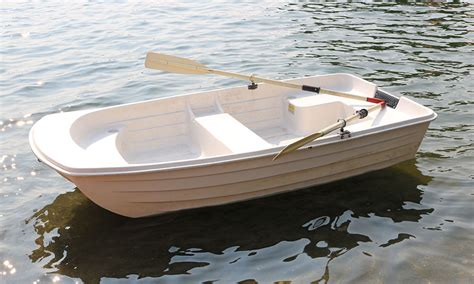
\includegraphics[width=\linewidth]{boat.jpeg}
      \caption{A boat.}
      \label{fig:boat1}
    \end{figure}

    \begin{figure}[h!]
      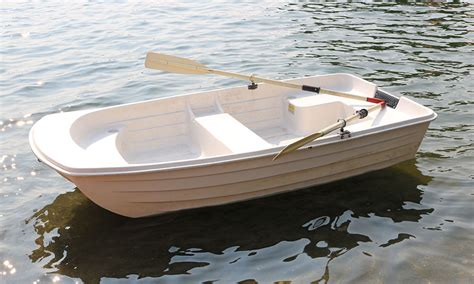
\includegraphics[width=\linewidth]{boat.jpeg}
      \caption{The same boat}
      \label{fig:boat2}
    \end{figure}

    \begin{figure}[b]
      \centering
      % These linewidth should be 0.1 less than what you expect
      \begin{subfigure}[b]{0.4\linewidth}
        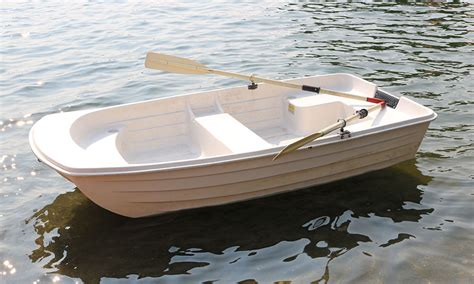
\includegraphics[width=\linewidth]{boat.jpeg}
        \caption{Boaty McBoatface.}
      \end{subfigure}
      \begin{subfigure}[b]{0.4\linewidth}
        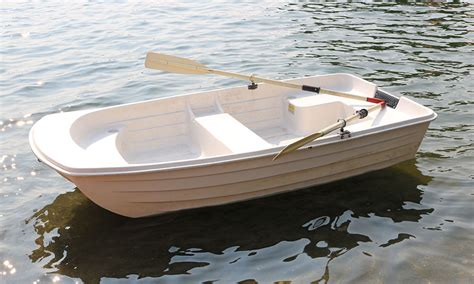
\includegraphics[width=\linewidth]{boat.jpeg}
        \caption{Boaty McBoatface 2.}
      \end{subfigure}
      \caption{An armada of boats.}
      \label{fig:boats}
    \end{figure}

    Figure \ref{fig:boat1} shows a boat.

  % ---------
  % Section 3
  % ---------
  \section{Tables}
    \begin{table}
      \caption{Dummy Table}
    \end{table}

  % ---------
  % Section 4
  % ---------
  \section{Citation Stuff and Footnotes}
    \subsection{Citation Stuff}
    Doing a book citation \autocite[31]{BOOK:1} here.
    And now it's time for an article citation \autocite[697]{ARTICLE:1}.
    Next up is another book \autocite[155]{BOOK:2} citation.
    Lastly, we have the website \autocite[]{WEBSITE:1} citation.

    \subsection{Footnotes}
    This is some example text\footnote{\label{myfootnote}Hello footnote}.

    \paragraph{A new Paragraph to mention the footnote.}
    Here I am mentioning a previous footnote, specifically I'm referring to this \ref{myfootnote} footnote.


  \newpage
  \printbibliography

  % --------
  % Appendix
  % --------
  \newpage
  \newpage
  \begin{appendix}
    \listoffigures
    \listoftables
  \end{appendix}

\end{document}